\chapter{Bitcoin, a peer-to-peer payment network}
\label{chap:bitcoin}

The Bitcoin ecosystem is composed of multiple actors. Users of the network access
information via wallets in their laptop or mobile phone. These users can see the amount
present in their addresses. An address is the representation of a public key, herself
being the representation of a private key. An address is own by a user if this user
has in his possession the associated private key. Users can transfer funds from some
of their addresses to other addresses own by other users or theirself. When funds
are transfered a transaction is created and send to the network. The network is
composed by nodes and these nodes take care of its proper functioning. Some of these
nodes are called miners, they listen to new transactions and try to include them into
the blockchain. This blockchain is the output, the intrinsec result, of the Bitcoin
protocol and can be compared to a distributed public ledger. Nodes are softwares
running all over the world, these softwares are maintained and improved by a group
of developers present all over the world and for Bitcoin, the original and reference
implementation is Bitcoin-core. The software allows to interact with the blockchain.
It is possible to retreive information such as current unconfirmed transactions,
information present in the blockchain, amount available for an address, etc.
An unconfirmed transaction is a transaction that has not been yet included into
the blockchain.

In the following some building blocks needed to figure out how payment channels works
and how we can improve them with some cryptography are traveled. If you are a master
of Bitcoin and you already know how blocks are created, how transactions are structured,
how fees are calculated and how segregated witness works, this chapter will be just
a reminder. For further explaination the best ressource today is the book \say{Mastering
Bitcoin} by Andreas Antonopoulos \cite{Antonopoulos:2014:MBU:2695500}.

% type of nodes in the peer-to-peer network
% \url{https://github.com/bitcoinbook/bitcoinbook/blob/second_edition/ch08.asciidoc}

\minitoc

\newpage

% -----------------------------------------------------------------------------
\section{The blockchain}

The blockchain, as indicated by his name, is a chain of blocks. Blocks are created
by the miners in a race to find the next valid block called the mining process. A block is considered valid
if its identifier, i.e. the double hash of its header, is lower to the current
difficulty target. It is worth noting that the validity of a block is based on multiple
other criterion who are not exposed here, for further information please refer
to the book \say{Mastering Bitcoin}. The header of a block is composed of a version
number, a creation timestamp, a nonce, or the difficulty target used as boundary.

The difficulty target is adjusted so a valid block is found in the network every
ten minutes in average. Mining can be modelized as a poisson process, i.e. the probability
of a given number of events occurring in a fixed interval of time or space if these
events occur with a known constant rate is independent of the time since the last event.
A miner will create a candidate block and compute its identifier, if this identifier
is lower than the current difficulty target then the block is valid and the miner notice
the network that he found the next block. Then the process start again. If the block
identifier is not valid the miner can change the nonce value in the header and
check with the new identifier. Finding the next valid block is so a computation that
require an enormous amount of power. All the network, round the clock, keeps searching
for the next valid block and the power of computation increase day after days.

\subsection{A chain of blocks}

As mentioned before, the blockchain is a chain who must be secure, verifiable,
and immutable. To achieve immutability, modification of previous blocks must
invalidate the chain. The block identifier is affected by information like the
creation timestamp or the nonce used to adapt the modifier but also from the
previous block identifier in the chain. That means that if the previous block
identifier is changed for exemple, because its content changed, the child block
into the chain will become invalid as well as its child, and so on.

Modifying the blockchain without invalidate the chain require to recompute all the
block identifiers after the changed block. This require a quantity of power that
can be estimated and for which the costs represent a certain safety threshold.
It is established that a transaction included in a block can be considered as safe
after six child blocks. The amount of power needed to erase this transaction became
statistically too high to be probable, but it does not means that it will never happen
due to the fact that there is the same probability to find a valid block with the
first nonce than with the thousandth.

\subsection{A list of transactions}

To be useful, a block needs a content. In Bitcoin the content of a block is composed
of transactions. As mentioned before, a transaction is called \textit{confirmed} when
she is included in a block. The number of confirmation is related to the number of
blocks mined after that the transaction has been included.

To keep track of all the transactions included into a block, a Merkle tree is created.
A Merkle tree or hash tree is a is a tree in which every leaf node is labelled with
the hash of a data block and every non-leaf node is labelled with the cryptographic
hash of the labels of its child nodes.

\begin{figure}[H]
	\centering
	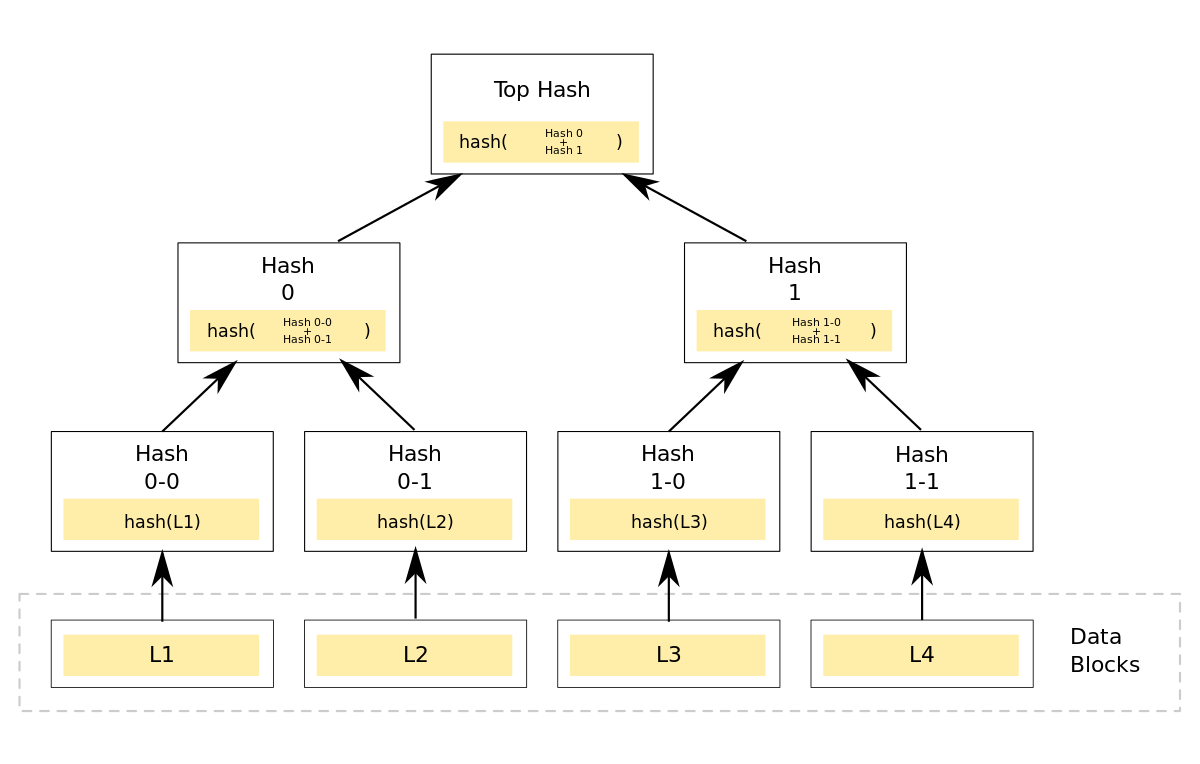
\includegraphics[width=1\columnwidth]{merkleTree}
	\captionsource{Merkle tree construction}{Merkle tree construction}
	{\url{https://en.wikipedia.org/wiki/Merkle_tree}}
	\label{fig:merkleTree}
\end{figure}

Given the top hash or Merkle root and a leaf, it is possible to prove the membership
by given the path for each complementary hashes. E.g given the Merkle root and \texttt{L1},
the proof is \texttt{Hash 0-1} and \texttt{Hash 1}. The verifier can then compute
the hash of \texttt{L1}, the result of this hash with \texttt{Hash 0-1}, and then with
\texttt{Hash 1}. If the result is the same as the Merkle root, then \texttt{L1} is a part
of the tree.

In a block, a Merkle tree of all included transaction identifiers is created. The
obtained Merkle root is put into the header of the block. To validate if a transaction
is included in a block the path must be given, then the resulting hash is compared
to the Merkle root registered in the block's header.

% -----------------------------------------------------------------------------
\section{Transactions}

% -- Your text goes here --

\subsection{A list of inputs \& outputs}

% -- Your text goes here --

\subsection{Segregated witness}

% -- Your text goes here --

\subsection{Scripting language}

% -- Your text goes here --
Locking script, unlocking script

\subsection{Transaction fees}

% -- Your text goes here --

% -----------------------------------------------------------------------------
\section{Scalability of Bitcoin}

% -- Your text goes here --

\subsection{On-chain improvements}
\subsection{Layer-two applications}
